% Bartosz Bednarczyk, Jan Góra
% Analiza numeryczna sprawozdanie

\documentclass{article}

\usepackage{polski}
\usepackage[utf8]{inputenc}

\usepackage{fancyhdr} % Required for custom headers
\usepackage{lastpage} % Required to determine the last page for the footer
\usepackage{extramarks} % Required for headers and footers
\usepackage[usenames,dvipsnames]{color} % Required for custom colors
\usepackage{graphicx} % Required to insert images
\usepackage{listings} % Required for insertion of code
\usepackage{courier} % Required for the courier font
\usepackage{lipsum} 
\usepackage{amsfonts}
\usepackage{amsthm}
\usepackage{hyperref}
\usepackage{tikz}
\usepackage{amsmath}
\usepackage{pdfpages}
\usepackage{mathtools}
\usepackage{amsthm}

\DeclareUnicodeCharacter{00A0}{ }

\newtheorem{thm}{Twierdzenie}
\newtheorem{remark}{Uwaga}
\newtheorem{lemat}{Lemat}
\newtheorem{wniosek}{Wniosek}
\newtheorem{definicja}{Definicja}
\newtheorem{ciekawostka}{Ciekawostka}
\newtheorem{przyklad}{Przykład}


\newenvironment{prooff}{\paragraph{Dowód:}}{\hfill$\square$}
\newenvironment{rozw}{\paragraph{Rozwiązanie:}}{\hfill}


\usepackage{inconsolata} % very nice fixed-width font included with texlive-full
\usepackage[usenames,dvipsnames]{color} % more flexible names for syntax highlighting colors
\usepackage{listings}

\lstset{
basicstyle=\small\ttfamily, 
columns=fullflexible, % make sure to use fixed-width font, CM typewriter is NOT fixed width
numbers=left, 
numberstyle=\small\ttfamily\color{Gray},
stepnumber=1,              
numbersep=10pt, 
numberfirstline=true, 
numberblanklines=true, 
tabsize=4,
lineskip=-1.5pt,
extendedchars=true,
breaklines=true,        
keywordstyle=\color{Blue}\bfseries,
identifierstyle=, % using emph or index keywords
commentstyle=\sffamily\color{OliveGreen},
stringstyle=\color{Maroon},
showstringspaces=false,
showtabs=false,
upquote=false,
texcl=true, % interpet comments as LaTeX
    literate={á}{{\'a}}1 {ã}{{\~a}}1 {é}{{<}}1,
inputencoding=utf8
}

\lstdefinelanguage{julia}
{
  keywordsprefix=\@,
  morekeywords={
    exit,whos,edit,load,is,isa,isequal,typeof,tuple,ntuple,uid,hash,finalizer,convert,promote,
    subtype,typemin,typemax,realmin,realmax,sizeof,eps,promote_type,method_exists,applicable,
    invoke,dlopen,dlsym,system,error,throw,assert,new,Inf,Nan,pi,im,begin,while,for,in,return,
    break,continue,macro,quote,let,if,elseif,else,try,catch,end,bitstype,ccall,do,using,module,
    import,export,importall,baremodule,immutable,local,global,const,Bool,Int,Int8,Int16,Int32,
    Int64,Uint,Uint8,Uint16,Uint32,Uint64,Float32,Float64,Complex64,Complex128,Any,Nothing,None,
    function,type,typealias,abstract
  },
  sensitive=true,
  morecomment=[l]{\#},
  morestring=[b]',
  morestring=[b]" 
}

% Margins
\topmargin=-0.45in
\evensidemargin=0in
\oddsidemargin=0in
\textwidth=6.5in
\textheight=9.0in
\headsep=0.25in

\linespread{1.1} % Line spacing

% Set up the header and footer
\pagestyle{fancy}
\lhead{\hmwkAuthorName} % Top left header
\rhead{\firstxmark} % Top right header
\lfoot{\lastxmark} % Bottom left footer
\cfoot{} % Bottom center footer
\rfoot{Page\ \thepage\ of\ \protect\pageref{LastPage}} % Bottom right footer
\renewcommand\headrulewidth{0.4pt} % Size of the header rule
\renewcommand\footrulewidth{0.4pt} % Size of the footer rule

\setlength\parindent{0pt} % Removes all indentation from paragraphs
%----------------------------------------------------------------------------------------
%	DOCUMENT STRUCTURE COMMANDS
%	Skip this unless you know what you're doing
%----------------------------------------------------------------------------------------

% Header and footer for when a page split occurs within a problem environment
\newcommand{\enterProblemHeader}[1]{
\nobreak\extramarks{#1}{#1 continued on next page\ldots}\nobreak
\nobreak\extramarks{#1 (continued)}{#1 continued on next page\ldots}\nobreak
}

% Header and footer for when a page split occurs between problem environments
\newcommand{\exitProblemHeader}[1]{
\nobreak\extramarks{#1 (continued)}{#1 continued on next page\ldots}\nobreak
\nobreak\extramarks{#1}{}\nobreak
}

\setcounter{secnumdepth}{0} % Removes default section numbers
\newcounter{homeworkProblemCounter} % Creates a counter to keep track of the number of problems

\newcommand{\homeworkProblemName}{}
\newenvironment{homeworkProblem}[1][Zadanie \arabic{homeworkProblemCounter}]{ % Makes a new environment called homeworkProblem which takes 1 argument (custom name) but the default is "Problem #"
\stepcounter{homeworkProblemCounter} % Increase counter for number of problems
\renewcommand{\homeworkProblemName}{#1} % Assign \homeworkProblemName the name of the problem
\section{\homeworkProblemName} % Make a section in the document with the custom problem count
\enterProblemHeader{\homeworkProblemName} % Header and footer within the environment
}{
\exitProblemHeader{\homeworkProblemName} % Header and footer after the environment
}

\newcommand{\problemAnswer}[1]{ % Defines the problem answer command with the content as the only argument
\noindent\framebox[\columnwidth][c]{\begin{minipage}{0.98\columnwidth}#1\end{minipage}} % Makes the box around the problem answer and puts the content inside
}

\newcommand{\homeworkSectionName}{}
\newenvironment{homeworkSection}[1]{ % New environment for sections within homework problems, takes 1 argument - the name of the section
\renewcommand{\homeworkSectionName}{#1} % Assign \homeworkSectionName to the name of the section from the environment argument
\subsection{\homeworkSectionName} % Make a subsection with the custom name of the subsection
\enterProblemHeader{\homeworkProblemName\ [\homeworkSectionName]} % Header and footer within the environment
}{
\enterProblemHeader{\homeworkProblemName} % Header and footer after the environment
}

\usepackage{listings} % Required for inserting code snippets
\usepackage[usenames,dvipsnames]{color} % Required for specifying custom colors and referring to colors by name

\definecolor{DarkGreen}{rgb}{0.0,0.4,0.0} % Comment color
\definecolor{highlight}{RGB}{255,251,204} % Code highlight color

% Create a command to cleanly insert a snippet with the style above anywhere in the document
\newcommand{\insertcode}[2]{\begin{itemize}\item[]\lstinputlisting[caption=#2,label=#1,style=Style1]{#1}\end{itemize}} % The first argument is the script location/filename and the second is a caption for the listing

%----------------------------------------------------------------------------------------
%	NAME AND CLASS SECTION
%----------------------------------------------------------------------------------------

\newcommand{\hmwkTitle}{Pracownia 1} % Assignment title
\newcommand{\hmwkDueDate}{} % Due date
\newcommand{\hmwkClass}{Analiza numeryczna} % Course/class
\newcommand{\hmwkClassTime}{} % Class/lecture time
\newcommand{\hmwkClassInstructor}{} % Teacher/lecturer
\newcommand{\hmwkAuthorName}{Bartosz Bednarczyk, Jan Góra - Sprawozdanie z pracowni nr 1 - Zadanie 24} % Your name

%----------------------------------------------------------------------------------------
%	TITLE PAGE
%----------------------------------------------------------------------------------------

\title{Analiza numeryczna (M) - Pracownia 1 - Zadanie P1.24\\
Analiza numeryczna iteracyjnej metody Bairstowa}
\date{Listopad 15, 2015}
\author{Bartosz Bednarczyk\\ \and Jan Góra}


%----------------------------------------------------------------------------------------

\begin{document}

\maketitle

\tableofcontents

\section*{Krótki opis sprawozdania}

Najprostsze metody numeryczne bardzo często okazują się być mało wydajne, dlatego matematycy dążą do uzyskania metod o bardzo niskim czasie działania. Celem tego sprawozdania jest pokazanie jednej z nich, jaką jest iteracyjna metoda Bairstowa. Na podstawie odpowiednich testów numerycznych sprawdzone zostaną dokładność, stabilność i efektywność tej metody. Poza tym pobieżnie omówione zostaną różne warianty metody Newtona, metoda Laguerre'a oraz metoda Mullera, których wydajność porównamy z metodą Bairstowa.	
\section{Przegląd podstawowych zagadnień związanych z wielomianami}

\subsection{Podstawowe definicje}

\begin{definicja}
Wielomianem stopnia $n \in \mathbb{N}$ nad ciałem $\mathbb{K}$ będziemy nazywać przekształcenie $\mathbb{K} \mapsto \mathbb{K}$ zadane wzorem $W(x) = a_0 + a_1x + \ldots + a_n x^n$, gdzie $a_i$ to pewne  współczynniki z ciała $\mathbb{K}$ oraz $a_n \neq 0$.
\end{definicja}

\begin{definicja}
Niech $W$ będzie pewnym wielomianem (nad ciałem $\mathbb{K}$). Liczbę $a$ taką, że $W(a) = 0$, będziemy nazywać pierwiastkiem wielomianu.
\end{definicja}

\begin{remark}
Z faktu, że wielomian $W$ ma współczynniki z ciała $\mathbb{K}$, nie wynika fakt, że jego pierwiastki również będą należeć do $\mathbb{K}$. Klasycznym przykładem jest wielomian $x^2 + 1$, który ma współczynniki rzeczywiste, a jego pierwiastkami są liczby zespolone.
\end{remark}

\begin{remark}
Istnieją takie ciała $\mathbb{K}$, że dla dowolnego wielomianu stopnia większego od $0$ wszystkie jego pierwiastki należą do $\mathbb{K}$. Ciała takie będziemy nazywać algebraicznie domkniętymi. Przykładem takiego ciała jest $\mathbb{C}$, czego nie będziemy dowodzić. 
\end{remark}

Podczas całego tego sprawozdania będziemy zajmować się następującym problemem:

\begin{center}
\begin{tikzpicture}
\node [draw={black}, fill=black!10, very thick, rectangle, rounded corners, inner sep=12pt, inner ysep=12pt] (box){%
    \begin{minipage}{.9\textwidth}

	Niech $W$ będzie wielomianem. Znaleźć zbiór $ker(W) = \lbrace a \ | \ W(a) = 0 \rbrace $.
    \end{minipage}
};
\node[fill={black}, text=white, rounded corners, right=10pt] at (box.north west) {Problem znajdowania miejsc zerowych wielomianu};
\end{tikzpicture}
\end{center}

Powyższy problem, choć pozornie prosty, jest sformułowany bardzo ogólnie. Na potrzeby tej pracy od tej pory ograniczymy się tylko do ciał $\mathbb{R}$ oraz $\mathbb{C}$, choć nic nie staje na przeszkodzie by poeksperymentować z innymi ciałami. Aktualnie nie wiemy czy każdy wielomian ma pierwiastki, a jeśli ma, to jaka jest moc ich zbioru. Nie znamy również żadnych metod rozwiązywania $W(x) = 0$. By lepiej zrozumieć podane zagadnienie, przejdźmy przez ciąg różnych definicji, algorytmów, twierdzeń i lematów związanych z wielomianami (warto je zrozumieć, gdyż kolejne rozdziały będą z nich korzystać).

\begin{thm}
Każdy wielomian $W(x)$ nad $\mathbb{C}$ stopnia $n \in \mathbb{N}_+$ ma co najmniej jeden pierwiastek.
\end{thm}

\begin{proof}
To twierdzenie jest nazywane zasadniczym twierdzeniem algebry. Udowodnione w \cite{leja}, s. 105.
\end{proof}

\begin{wniosek}
$| ker(W) | \leq n$, gdzie $n$ to stopień wielomianu $W$.	
\end{wniosek}


\subsection{Postać iloczynowa wielomianu i dzielenie wielomianu}


\begin{definicja}
Wielomian $W(x)$ nazywamy podzielnym przez wielomian $P(x)$, różny od wielomianu zerowego, wtedy i tylko wtedy, gdy istnieje taki wielomian $Q(x)$, że $W(x) = Q(x) \cdot P(x)$. Wielomian $Q(x)$ nazywamy ilorazem wielomianu $W(x)$ przez $P(x)$. Mówimy, że wielomian $P(x)$ jest dzielnikiem wielomianu $W(x)$.
\end{definicja}


\begin{thm}
Dowolny wielomian $W(x)$ możemy zapisać jako $W(x) = P(x) \cdot Q(x) + R(x)$ dla pewnych wielomianów $P, Q, R$. Mówimy, że wielomian $W(x)$ jest podzielny przez $Q(x)$, jeżeli $R(x) = 0$. 
\end{thm}

\begin{thm}
Wielomian $W(x)$ jest podzielny przez wielomian $Q(x) = (x-a)$ wtedy i tylko wtedy, gdy $W(a) = 0$.	
\end{thm}

\begin{proof}
Udowodnione w \cite{kostrikin}, s. 198-199.
\end{proof}

Chcielibyśmy umieć w efektywny sposób realizować procedurę dzielenia wielomianu przez jednomiany postaci $x-a$. Służy do tego następujący algorytm:

\begin{enumerate}
\item $P(x) = a_0 + a_1 x + a_2 x^2 + \ldots + a_n x^n$.
\item Niech $\alpha = a_n$.
\item Kolejno dla $k = n-1, n-2, \ldots 0$ wykonaj $\alpha := a_k + x \alpha$.
\item Wynik to $p(x) = \alpha$.
\end{enumerate}

Dokładny opis metody oraz jej analizę możemy znaleźć w \cite{kincaid}, s. 103.\\

\subsection{Pochodna wielomianu i jej obliczanie}

\begin{definicja}
Pochodną wielomianu $p(x) = a_nx^n + a_{n-1}x^{n-1} + \ldots + a_1x + a_0$ będziemy nazywać wielomian $p'(x) = 	n \cdot a_n x^{n-1} + (n-1) a_{n-1}x^{n-2} + \ldots +  a_1$.
\end{definicja}

Wyznaczanie wielomianu w punkcie $x_0$ możemy zrealizować za pomocą schematu Hornera:

\begin{enumerate}
\item $P(x) = a_0 + a_1 x + a_2 x^2 + \ldots + a_n x^n$.
\item Niech $\alpha := a_n, \ \beta := 0$.
\item Kolejno dla $k = n-1, n-2, \ldots 0$ wykonaj $\beta := \alpha + x \beta, \ \alpha := a_k + x \alpha.$

\item Wynik to $p'(x) = \beta$.
\end{enumerate}

\subsection{Inne przydatne pojęcia matematyczne}

Oprócz wymienionych w rozdziale pojęć związanych z wielomianami, zakładać będziemy u czytelnika znajomość wielowymiarowego rachunku różniczkowego, definicji funkcji holomorficznej oraz podstawowych pojęć związanych z analizą błędów. Pojęcia te można doczytać w \cite{leja} i \cite{kincaid}. 

\section{Metoda Newtona oraz wielowymiarowa metoda Newtona}

\subsection{Opis klasycznej metody Newtona}

Klasyczną metodą Newtona zastosowaną dla pewnego punktu startowego $p$ oraz funkcji $f : \mathbb{R} \mapsto \mathbb{R}$ klasy $C^{1}$ nazywać będziemy metodę iteracyjną postaci:

$$
x_n = \left\{\begin{matrix}
p, & gdy \ n = 0\\ 
x_{n-1} - \frac{f(x_{n-1})}{f'(x_{n-1})}, & w.p.p. 
\end{matrix}\right.
$$

Można pokazać, że $x_n$ zbiega do pewnego pierwiastka funkcji $f$. Analizę klasycznej metody Newtona można znaleźć w \cite{kincaid}, s.   71-81.

\subsection{Zastosowanie klasycznej metody Newtona do szukania zer wielomianu}

Jeśli mamy wielomian o współczynnikach i pierwiastkach rzeczywistych, możemy policzyć jego pierwiastki za pomocą klasycznej metody Newtona. Podstawiamy za $f$ z poprzedniego opisu nasz wielomian, a $f'$ to jego pochodna. Po znalezieniu jednego pierwiastka (nazwijmy go $a$) dzielimy nasz wielomian przez $x-a$ i uruchamiamy program dla otrzymanego wielomianu. Proces kontynuujemy tak długo, aż dojdziemy do wielomianu o stopniu $0$.

\begin{remark}
Poniżej przedstawiamy przykładową implementację metody Newtona w języku Julia. Wartość w punkcie wielomianu i jego pochodnej możemy wyznaczyć z pomocą schematu Hornera, który był omówiony wcześniej (w kodzie przykładowym skorzystaliśmy z funkcji bibliotecznych dla większej czytelności).
\end{remark}


\lstset{language=Julia, label=DescriptiveLabel, frame=shadowbox}
\lstinputlisting{klasyczna_metoda_newtona.jl}

\begin{remark}
Powyższa metoda nie nadaje się do obliczania miejsc zerowych wielomianu, którego pierwiastki są zespolone (z powodu tego, że operujemy tutaj na tylko rzeczywistych przybliżeniach $x_n$).
\end{remark}

\subsection{Metoda Newtona dla wielu funkcji wielu zmiennych}

Załóżmy, że mamy do rozwiązania układ równań:

$$\left\{\begin{matrix}
f_1(x_1, x_2, \ldots, x_n) = 0 \\ 
f_2(x_1, x_2, \ldots, x_n) = 0 \\ 
\ldots\\ 
f_n(x_1, x_2, \ldots, x_n) = 0,
\end{matrix}\right.$$

gdzie $f_i \in \mathbb{R}^n \mapsto \mathbb{R}^n$ jest klasy $C^{1}$.

Każdą z tych funkcji możemy rozpisać ze wzoru Taylora jako:

$$0 = f_i(x_1 + h_1, x_2 + h_2, \ldots, x_n + h_n) \approx f_i(x_1, x_2, \ldots, x_n) + \sum_{j=1}^n h_j \cdot \frac{\partial f_i}{\partial x_j} (x_1, x_2, \ldots x_n)$$

Powyższy układ możemy zapisać w postaci macierzowej:

$$
\begin{pmatrix}
f_1(x_1, x_2, \ldots, x_n)\\ 
f_2(x_1, x_2, \ldots, x_n)\\ 
\ldots\\ 
f_n(x_1, x_2, \ldots, x_n)\\ 

\end{pmatrix} = \begin{pmatrix}
\frac{\partial f_1}{\partial x_1}(x_1, x_2, \ldots x_n) & \frac{\partial f_1}{\partial x_2}(x_1, x_2, \ldots x_n) &  \ldots &  & \frac{\partial f_1}{\partial x_1}(x_1, x_2, \ldots x_n) \\ 
\frac{\partial f_2}{\partial x_1}(x_1, x_2, \ldots x_n) & \frac{\partial f_2}{\partial x_2}(x_1, x_2, \ldots x_n) &  \ldots &  & \frac{\partial f_2}{\partial x_1}(x_1, x_2, \ldots x_n) \\ 
 \ldots & \ldots &  \ \ldots & \\ 
 \ldots & \ldots &  \ \ldots & \\ 
\frac{\partial f_n}{\partial x_1}(x_1, x_2, \ldots x_n) & \frac{\partial f_n}{\partial x_2}(x_1, x_2, \ldots x_n) &  \ldots &  & \frac{\partial f_n}{\partial x_1}(x_1, x_2, \ldots x_n) \\ 
\end{pmatrix} \begin{pmatrix}
h_1\\ 
h_2\\ 
\ldots \\ 
\ldots \\ 
h_n\\ 

\end{pmatrix}
$$

Aby nieco skrócić ten układ, będziemy go zapisywać jako $F(X) = -J \cdot H$.
Jeśli macierz $J$ jest nieosobliwa, to układ ma rozwiązanie w postaci:
$$ -J^{-1} \cdot F(X) = H$$

Ostatecznie wzór Newtona dla układu funkcji wielu zmiennych możemy wyrazić wzorem:

$$ X_{k+1} = X_k + H_k = X_k - J^{-1}(X_k) F(X_k)$$


\subsection{Metoda Newtona dla funkcji zespolonych}

\begin{lemat}
Dowolną funkcję analityczną $f : \mathbb{C} \mapsto \mathbb{C}$ możemy zapisać jako $$f(z) = f(x+yi) = P(x,y) + i Q(x,y),$$ gdzie $x,y \in \mathbb{R}$, $P(x,y) \in \mathbb{R}, Q(x,y) \in \mathbb{R}$	
\end{lemat}

\begin{przyklad}

$$f(z) = z^3 - 2z = f(x+iy) = (x+iy)^3 - 2(x+iy) = (x^3 - 3xy^2 - 2x) + i(3x^2y - y^3 - 2y) = P(x,y) + iQ(x,y)$$

\end{przyklad}


Niech $f(z) = P(x,y) + iQ(x,y)$. Równanie $f(z) = 0$ możemy sprowadzić do układu równań $Q(x,y) = 0$ i $P(x,y) = 0$. Taki układ równań rozwiązujemy za pomocą metody Newtona dla funkcji wielu zmiennych.

$$v_{n+1} = v_n - \frac{f(v_n)}{f'(v_n)}$$

$$
\begin{pmatrix} x_{n+1}\\ y_{n+1}\\ \end{pmatrix} =  \begin{pmatrix} x_n\\ y_n\\ \end{pmatrix} - J^{-1} \begin{pmatrix} P(x_n, y_n)\\ Q(x_n, y_n)\\ \end{pmatrix} = 
\begin{pmatrix} x_n\\ y_n\\ \end{pmatrix} - \begin{pmatrix}
\frac{\partial P}{\partial x}(x_n, y_n) & \frac{\partial P}{\partial y} (x_n, y_n)\\ 
\frac{\partial Q}{\partial x}(x_n, y_n) & \frac{\partial Q}{\partial y}(x_n, y_n)  
\end{pmatrix}^{-1} \begin{pmatrix} P(x_n, y_n)\\ Q(x_n, y_n)\\ \end{pmatrix} $$


Ponieważ wielomian jest funkcją holomorficzną, to zachodzi równanie Cauchy'ego-Riemanna:

$$\frac{\partial P}{\partial x} = \frac{\partial Q}{\partial y}, \ - \frac{\partial P}{\partial y} =\frac{\partial Q}{\partial x}$$

Oznaczając $P = P(x_n, y_n), Q = Q(x_n, y_n), P_x = \frac{\partial P}{\partial x}(x_n, y_n)$, $Q_x = \frac{\partial Q}{\partial x}(x_n, y_n)$ oraz korzystając ze wzoru na macierz odwrotną możemy uprościć wzór na metodę Newtona do postaci:

$$
\begin{pmatrix} x_{n+1}\\ y_{n+1}\\ \end{pmatrix} = \begin{pmatrix} x_n - \frac{ P P_x + Q Q_x}{Px^2 + Qx^2}\\ y_n - \frac{P P_y + Q Q_y}{Px^2 + Qx^2} \\ \end{pmatrix}
$$


\begin{remark}
Implementacja zespolonej metody Newtona jest nieco problematyczna. Musimy potrafić zaimplementować operacje na funkcjach wielu zmiennych oraz ich różniczkowanie. Przykładowy kod w języku Julia możemy otrzymać dzięki zastosowaniu biblioteki MultiPoly. Wymieniona biblioteka dostarcza nam sposobu na tworzenie nowych zmiennych wielomianu (metoda generators), obliczania wartości w danym punkcie (evaluate) oraz efektywnego różniczkowania wielomianu po zadanej zmiennej (diff).  \end{remark}


\lstset{language=Julia, label=DescriptiveLabel, frame=shadowbox}
\lstinputlisting{zespolony_newton.jl}

\section{Wybrane metody wyszukiwania miejsc zerowych wielomianu}

\subsection{Metoda Laguerre'a}

Jedną z metod iteracyjnych wyszukiwania pierwiastków wielomianu używanych w nowoczesnych systemach informatycznych jest metoda Laguerre'a. 

Niech $p(z)$ będzie wielomianem stopnia $n$, którego pierwiastki mamy znaleźć. Kolejne kroki w metodzie wykonujemy za pomocą nastepujących wzorów:

$$ A = \frac{-p'(z)}{p(z)}, \ B = A^2 - \frac{p''(z)}{p(z)}, \ C = \frac{A \pm \sqrt{(n-1)(nB - A^2}}{n}, \ z_{nowe} = z + \frac{1}{C}$$ 

Metoda Laguerre'a jest bardzo efektywnym algorytmem, ponieważ w okolicach pojedynczego pierwiastka wielomianu $p$ jest zbieżna sześcienne. Dokładną analizę tej metody pozostawiamy czytelnikowi do przeczytania w \cite{kincaid}, s. 112-116.

\subsection{Metoda Mullera}

Metoda Mullera jest modyfikacją metody stycznych. Zamiast przybliżać nasz wielomian $f$ funkcją liniową, będziemy go aproksymować funkcją kwadratową.

Rozważmy trzy punkty $x_0, x_1, x_2$ wraz z wartościami funkcji $f$ w tych punktach. Przyjmujmy, że $x_2$ jest aktualnym przybliżeniem rozwiązania. Oznaczmy $z = x-x_2, \ h_0 = x_0 - x_2, \ h_1 = x_1-x_2$.

Oznaczmy szukaną parabolę przez $g(z) = az^2 + bz + c$. Z definicji paraboli w punkcie $z - x_k$ dostajemy, że 

$$2a = f''(x_k), \ b = f'(x_k), \ c = f(x_k),$$

co prowadzi do wzoru

$$x_{k+1} = x_k - \frac{2f(x_k)}{f'(x_k) + sgn(f'(x_k)) \cdot \sqrt{(f'(x_k))^2 - 2f(x_k)f''(x_k)}}$$

Więcej na temat tej metody oraz jej modyfikacji można poczytać w skrypcie \cite{tajewski}.


\section{Metoda Bairstowa}

\subsection{Opis metody Bairstowa}

Ostatnią i zarazem najważniejsza metodą, którą omówimy w sprawozdaniu, będzie metoda Bairstowa. Wiemy, że nawet jeśli wielomian ma współczynniki rzeczywiste, to może mieć pierwiastki zespolone (np. $x^2 + 1$). Metoda Bairstowa pozwala na obliczenie wszystkich pierwiastków bez użycia arytmetyki zespolonej.


\begin{lemat}
Jeżeli $w$ jest pierwiastkiem nierzeczywistym wielomianu $p(z)$, a $p(z)$ jest wielomianem o współczynnikach rzeczywistych, to pierwiastkiem $p(z)$ jest również $\overline{w}$. Iloczyn $(x-w)(x-\overline{w})$ jest czynnikiem kwadratowym o współczynnikach rzeczywistych.
\end{lemat}

\begin{proof}
Udowodnione w \cite{kincaid}, s. 108.	
\end{proof}

Zauważmy, że pierwiastki zespolone możemy wyszukiwać parami. Zamiast wyszukiwać pierwiastki pojedynczo, będziemy wyszukiwać dwumianu postaci $z^2 - uz - v$.

\begin{lemat}
Dowolny wielomian $p(z) = a_nx^n  + a_{n-1}x^{n-1} + \ldots a_0$ możemy zapisać w postaci: 

$$p(z) = \left(b_nx^{n-2} + b_{n-1}z^{n-3} + \ldots + b_3 z + b_2 \right) \left( z^2 - uz - v \right) + b_1(z-u) + b_0 $$	

Wielomian $ \left(b_nx^{n-2} + b_{n-1}z^{n-3} + \ldots + b_3 z + b_2 \right) $ będziemy dalej oznaczać jako $Q(z, u, v)$.
Powyższe współczynniki możemy obliczać rekurencyjnie według wzorów:
$$b_{n+1} = b_{n+2} = 0, \ \ b_k = ub_{k+1} + vb_{k+2} \ (n \geq k \geq 0).$$

\end{lemat}

\begin{proof}
Dowód w \cite{kincaid}, s. 109.	
\end{proof}

Chcemy, by nasz wyjściowy wielomian był podzielny przez $z^2 - uz - v$. Zatem musi zachodzić $b_0 = b_1 = 0$. Potraktujmy podane współczynniki jako funkcje zmiennych $u,v$. Wtedy dostajemy do rozwiązania układ równań:
$$
\left\{\begin{matrix}
b_0(u + h_1, v + h_1) = 0 & \\ 
b_1(u + h_2, v + h_2) = 0 & 
\end{matrix}\right.
$$

Podany układ możemy rozwiązać przedstawioną wcześniej metodą Newtona dla wielu funkcji wielu zmiennych. Po znalezieniu współczynników $u, v$ dzielimy wyjściowy wielomian przez otrzymany dwumian i kontynuujemy proces wyszukiwania pierwiastków dla mniejszego wielomianu (z uwzględnieniem tego, że przypadki dla wielomianu stopnia $0$ i $1$ traktujemy osobno).

\subsection{Analiza teoretyczna metody Bairstowa}

\begin{lemat}
Metoda Bairstowa jest zbieżna lokalnie.	
\end{lemat}

\begin{proof}
Wynika to bezpośrednio z tego, że metoda Newtona jest zbieżna lokalnie.	
\end{proof}

Głównym założeniem w lokalnej zbieżności metody Bairstowa jest to, że jakobian wyliczany przy metodzie Newtona się nie zeruje dla podanych wcześniej punktów startowych i kolejnych przybliżeń. Zastanówmy się w jaki sposób zerowanie się jakobianu zależy od punktów startowych oraz pierwiastków wielomianu.

\begin{thm}
Niech $u, v$ będą dowolnie wybranymi liczbami rzeczywistymi. Jakobian dla algorytmu Bairstowa jest macierzą odwracalną wtedy i tylko wtedy, gdy $z^2 - uz - v$ oraz wielomian $Q(z,u,v)$ nie mają wspólnych pierwiastków. Rząd jakobianu jest jeden wtedy i tylko wtedy, kiedy liczba wspólnych pierwiastków (z krotnościami) jest równa jeden. Jakobian się zeruje wtedy i tylko wtedy, gdy $z^2 - uz - z$ dzieli $Q(z,u,v)$.
\end{thm}

\begin{thm}
Załóżmy, że $P(z) = Q(z, u, v) (x^2 - u^{\star} z - v^{\star})$ i załóżmy, że wyrażenia po prawej stronie nie mają wspólnego pierwiastka. Wtedy istnieje dodatnia liczba $d$ taka, że ciąg $(u_k, v_k)$ generowany przez metodę Bairstowa jest zbieżny kwadratowo do $(u^{\star}, v^{\star})$, gdzie $|u_0 - u^{\star}| < d \wedge |v_0 - v^{\star}| < d$. 
\end{thm}

\begin{proof}
Twierdzenia te zostały udowodnione przez autorów Tibora Fialę oraz Annę Krebsz w 1987 roku. Kompletne dowody można przeczytać w \cite{krebsz}.
\end{proof}

Analiza zbieżności oraz rozbieżności metody Bairstowa stanowiła podstawę do napisaniu kilku (choć niestety niewielu) prac naukowych. Zainteresowanego czytelnika odsyłamy do \cite{krebsz}, \cite{Gabler} oraz \cite{Glasson}. 

\subsection{Przykład rozbieżności metody Bairstowa}

Rozważmy wielomian postaci $P(x) = (x^2 + ux + v)(x^2 + ux + w) + (w-v)^2.$
Jakobian dla metody Bairstowa w punkcie $(u,v)$ będzie wyglądał następująco:
$$
J(u,v) = \begin{pmatrix}
v-w & 0\\ 
0 & v-w 
\end{pmatrix}
$$

Jeśli uruchomimy metodę Bairstowa dla np. $u = 3, v = 1, w = 2$ to dostaniemy wielomian $x^4 + 6x^3 + 12x^2 + 9x +3,$ dla którego ciąg przybliżeń pierwiastka będzie cykliczny.

\begin{table}[h!]
\centering
\caption{Metoda Bairstowa dla powyższej funkcji}
\label{my-label}
\begin{tabular}{|l|l|l|l|l|}
\hline
Iteracja & $x_0$           & $x_1$               & $x_2$           & $x_3$              \\ \hline
1        & -2.6180339884   & -3.8196601113e-01   & -2.6180339884   & -3.8196601113e-01   \\ \hline
2        & -2.0            & -1.0                & -2.0            & -1.0                \\ \hline
3        & -2.6180339884 & -3.8196601113e-01 & -2.6180339884 & -3.8196601113e-01 \\ \hline
4       & -2.0            & -1.0                & -2.0            & -1.0                \\ \hline

\end{tabular}
\end{table}

\subsection{Implementacja metody Bairstowa}

Jeżeli oznaczymy sobie $c_k := \frac{\partial b_k}{\partial u}, \ d_k := \frac{\partial b_{k-1}}{\partial v}$ to dostajemy związki:

$c_k = d_{k+1} + uc_{k+1} + vc_{j+2} \ (c_{n+1} = c_n = 0)$ oraz $d_k = b_{k+1} + u d_{k+1} + v d_{k+2} (d_{n+1} = d_n = 0)$.

Rozwiązujemy układ równań

$$
\left\{\begin{matrix}
b_0(u, v) + \frac{\partial b_0}{\partial u} \delta u + \frac{\partial b_0}{\partial v} \delta v  = 0 & \\ 
b_1(u, v) + \frac{\partial b_1}{\partial u} \delta u + \frac{\partial b_1}{\partial v} \delta v  = 0 & \\ \end{matrix}\right.
$$

Rozwiązaniem powyższego układu jest 
$$\delta u = (c_1b_1 - c_2b_0)/J, \ \delta v = (c_1 b_0 - c_0 b_1)/J, \ J = c_0c_2 - c_1^2$$

Metodę Bairstowa możemy zapisać w postaci listy kroków:

\begin{enumerate}
\item $b_n := a_n$
\item $c_n := 0$
\item $c_{n-1} := a_n$
\item for $j = 1$ to $M$ do
	\begin{enumerate}
	\item $b_{n-1} := a_{n-1} + ub_n$
	\item for $k = n-2$ to $0$ step $-1$ do
		\begin{enumerate}
		\item $b_k := a_k + ub_{k+1} + vb_{k+2}$
		\item $c_k := b_{k+1} + uc_{k+1} + vc_{k+2}$
		\end{enumerate}
	\item end do

\item $J := c_0c_2 - c_1^2$
\item $u := u + (c_1b_1 - c_2b_0)/J$
\item $v := v + (c_1b_0 - c_0b_1)/J$
\item output $j, u, v, b_0, b_1$
\end{enumerate}
\item end do	
\end{enumerate}

Pseudokod zapożyczony z opisu metody Bairstowa z \cite{kincaid}.

\subsection{Proponowane usprawnienia}

\begin{itemize}
\item W przypadku, kiedy po podanej liczbie iteracji nasz $(u, v)$ nie "wyzerował" dostatecznie współczynników $b_0$ oraz $b_1$ to możemy wylosować nowy punkt startowy $(u^{\star}, v^{\star})$ i zacząć metodę od początku. Ominiemy wtedy przypadek, że dla podanych początkowych punktów metoda się zapętla (patrz: s. $7$).

\item Jeżeli w danej iteracji jakobian się zeruje, a $b_1, b_0$ nie są "wyzerowane", to możemy również wylosować nowy punkt i zacząć metodę od początku.
	
\end{itemize}



\section{Testy numeryczne}

\subsection{Porównanie opisanych metod}

Poniższe wykresy prezentują obserwację zmiany błędu bezwzględnego pierwiastka wielomianu i przybliżenia zadanego przez opisaną metodą w kolejnych iteracjach na podstawie różnych danych wejściowych. Na wykresie oś Y przedstawia błąd bezwzględny w postaci $10^{-y}$.

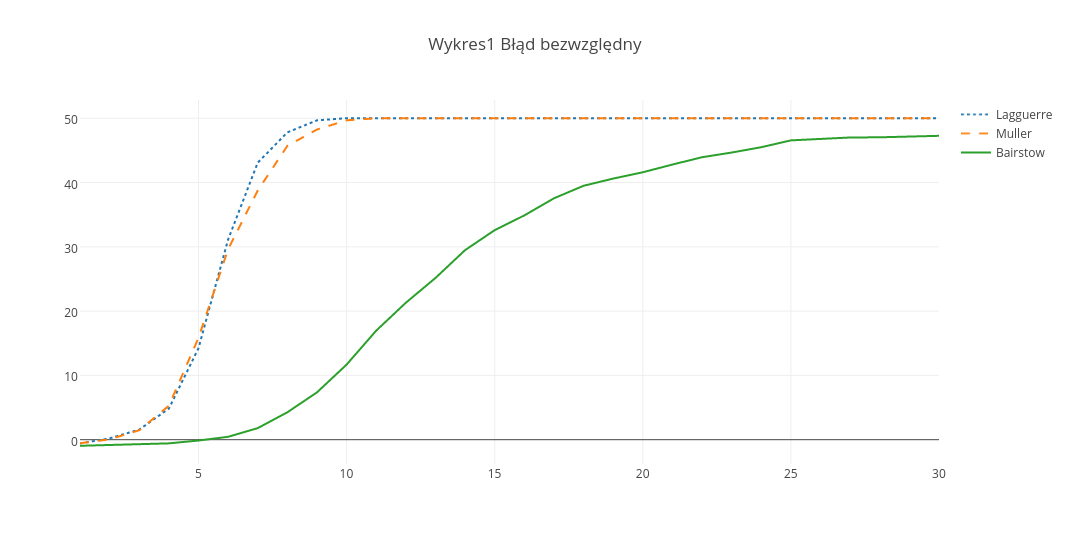
\includegraphics[scale=0.45]{w1.png}

Wykres 1:
Próba $100$ wielomianów $10$-tego stopnia o losowych pierwiastkach typu $BigFloat$ (o precyzji $10^{-30}$) w zakresie $[-7;7]$ w zerowych punktach początkowych.

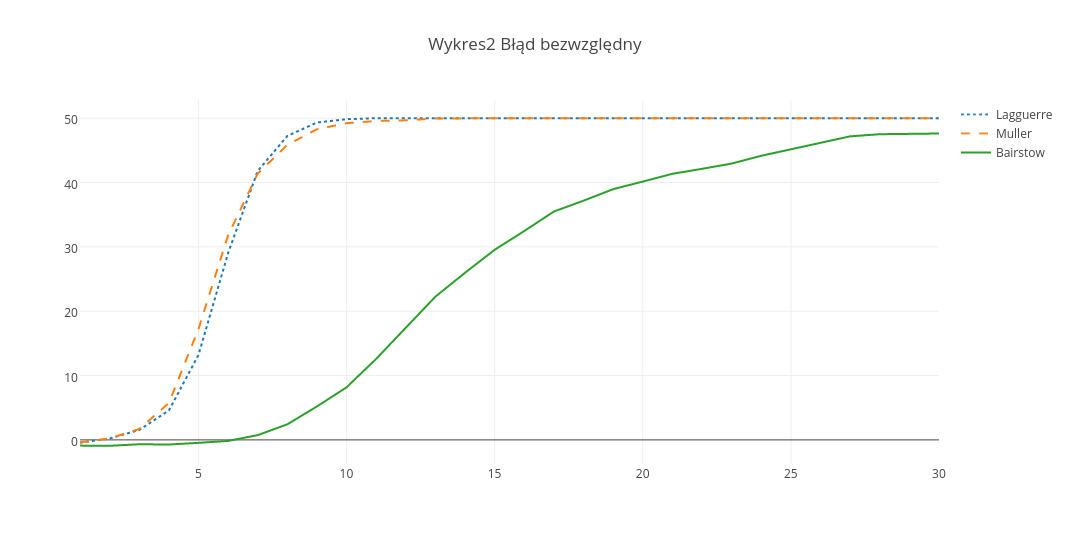
\includegraphics[scale=0.45]{w2.png}

Wykres 2:
Próba $100$ wielomianów $10$-tego stopnia o losowych pierwiastkach typu $BigFloat$ (o precyzji $10^{-30}$) w zakresie $[-7;7]$ w zerowych punktach początkowych.


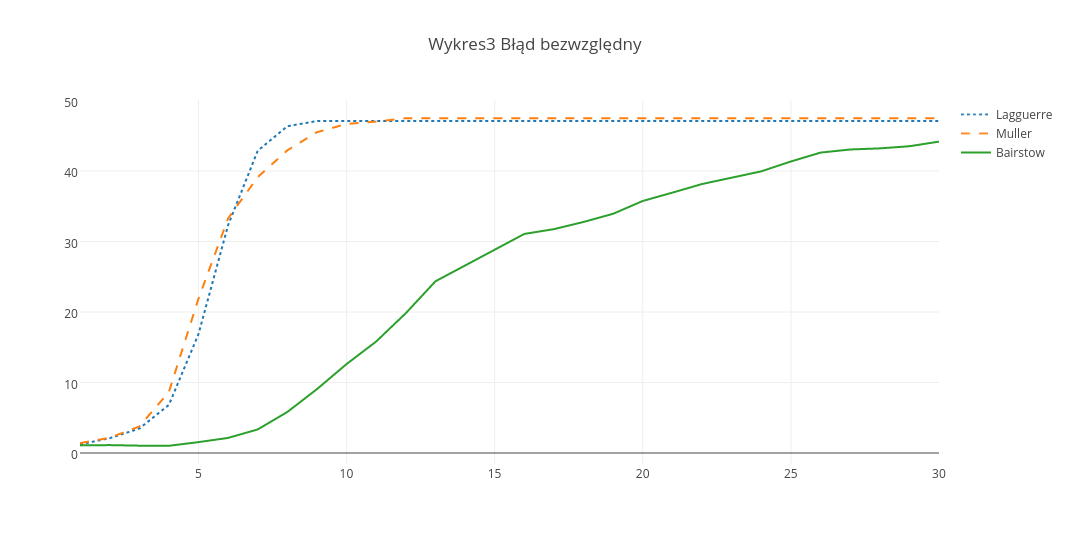
\includegraphics[scale=0.45]{w3.png}

Wykres 3:
Próba $50$ wielomianów $10$-tego stopnia o losowych pierwiastkach typu  $BigFloat$ (o precyzji $10^{-30}$) w zakresie $[0;1)$ w zerowych punktach początkowych.

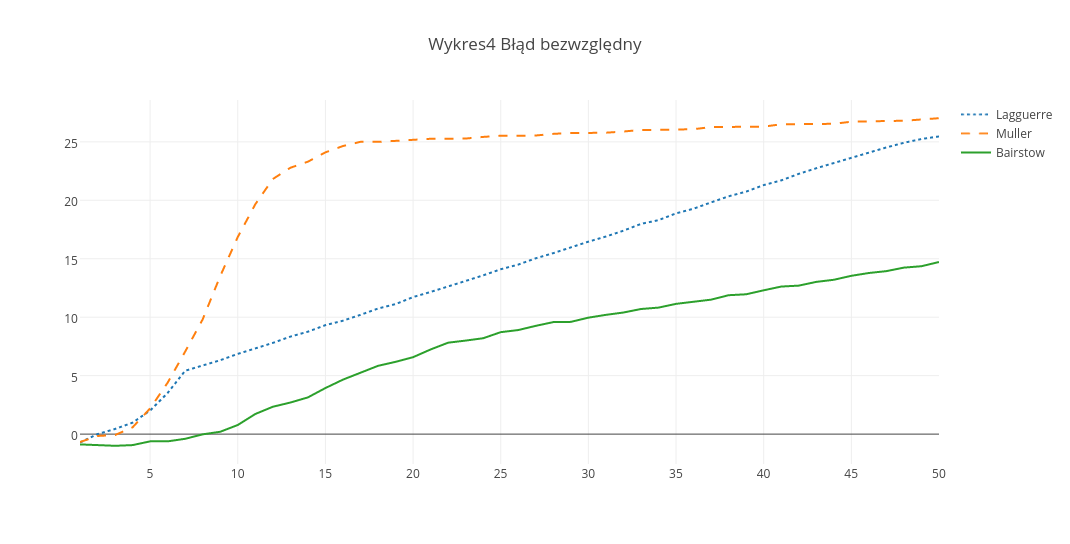
\includegraphics[scale=0.45]{w4.png}

Wykres 4:
Próba $50$ wielomianów $10$-tego stopnia o losowych pierwiastkach typu $Int64$ w zakresie $[-10;10]$ w zerowych punktach początkowych.

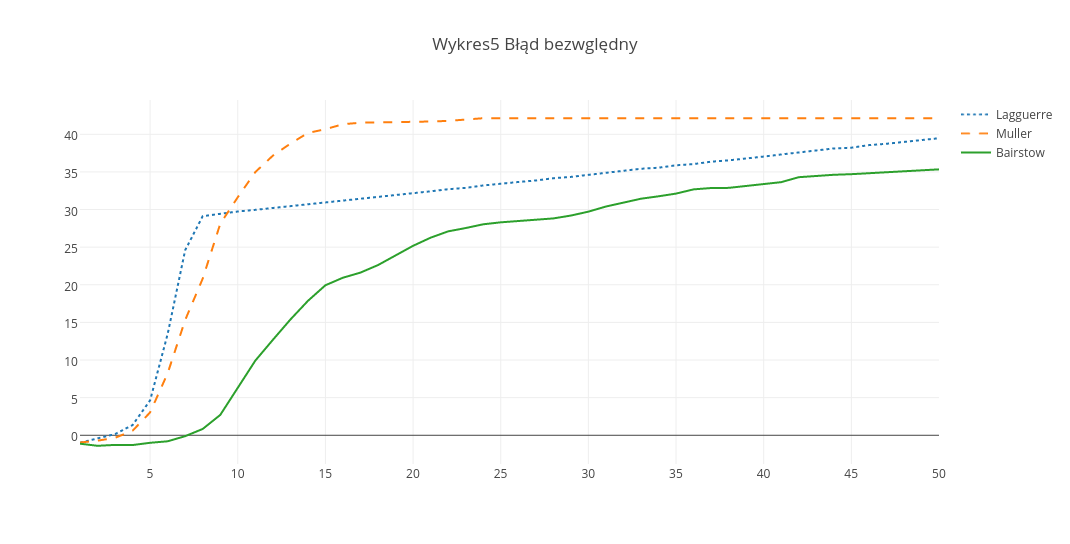
\includegraphics[scale=0.45]{w5.png}

Wykres 5:
Próba $50$ wielomianów $10$-tego stopnia o losowych pierwiastkach typu $Int64$ w zakresie $[-30,30]$ w zerowych punktach początkowych.

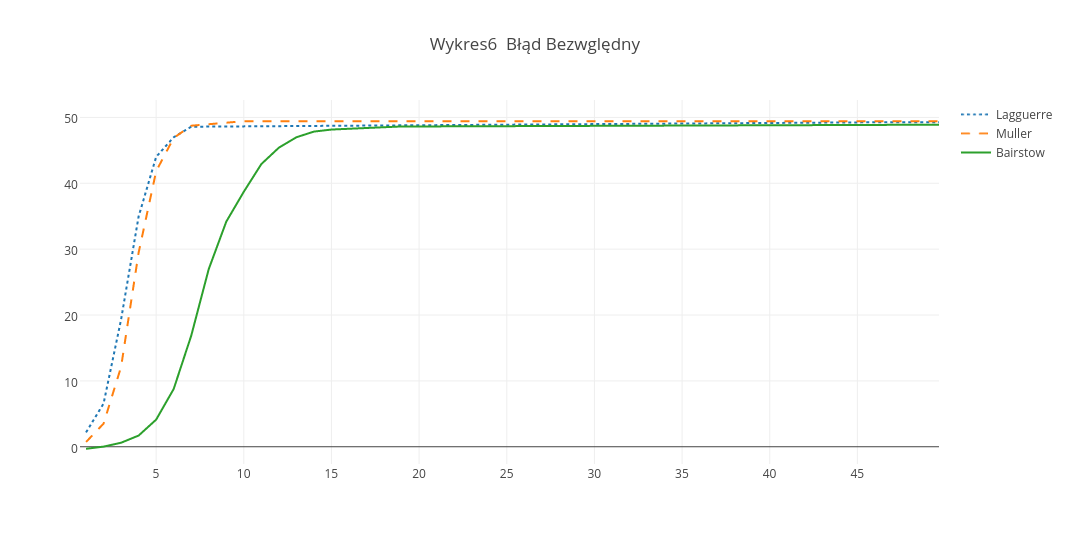
\includegraphics[scale=0.45]{w6.png}

Wykres 6:
Próba $50$ wielomianów $3$-tego stopnia o losowych pierwiastkach typu $Int64$ w zakresie $[-30;30]$ w zerowych punktach początkowych.

\pagebreak

\begin{wniosek}
Wykresy $1$ i $2$ oparte były na podobnych danych. Zauważamy, że funkcje na różnych wielomianach o tym samym typie zbiegają mniej-więcej w tej sam sposób. Widzimy, że metoda Bairstowa jest zdecydowanie wolniej zbieżna od dwóch pozostałych metod.\\

Na wykresie $3$ widać, że pomimo pozornie bliskich pierwiastków wielomianu ($[0,1)$) metody są równie szybko zbieżne.\\

Na wykresie $4$ widzimy, że bliskie pierwiastki są dużym utrudnieniem dla metod.
Błąd bezwzględny przy $50$ iteracjach nie przekroczył $10^{-30}$, podczas gdy w poprzednich przykładach już po $30$ iteracjach metody osiągnęły maksymalną dokładność.\\

Po zwiększeniu przedziału do $[-30;30]$ metody znów szybko osiągnęły dobrą dokładność.\\

Ostatni wykres prezentuje zachowanie metod na bardzo małych danych wejściowych. Widać, że wszystkie metody są bardzo szybko zbieżne.

\end{wniosek}

\subsection{Przykład działania opisanych metod}

\begin{przyklad}
Metoda Bairstowa zastosowana do wielomianu $$168 + 10x - 37x^2 + 2x^3 + x^4 = (x+2)(x-3)(x+7)(x-4)$$

\begin{enumerate}
\item Iteracja nr $1$:

$$-1.917879829307739159294843574606, \
2.441230459404106839057630824421,$$
$$-7.164414002968976450250192381454, \
5.164414002968976450250192381454$$	

\item Iteracja nr $2$:

$$-2.009530033377617967339383794074, \
2.900360110039499302979214698574
$$$$-6.970374011038727308629332841661,  \ 
4.447023380942359628866545591846
$$

\item Iteracja nr $3$:

$$
-2.001038440292382015085002297150, \
2.994714506062211330442943300673
$$
$$
-6.984875797781202526521865011540, \
4.094045721119321190882034107040
$$

\item Iteracja nr $4$:

$$
-2.000004229190859710286686827364, \
2.999983492821811977876729816709$$
$$-6.998950445144011486784616660300, \
4.005274379374182171426675656777$$


\item Iteracja nr $5$:

$$-2.000000000049071271087627181384, \ 
2.999999999847921708048370785679$$
$$-6.999996192489175048447504955397, \ 
4.000016928858222780857461966052
$$

\item Iteracja nr $6$:

$$-2.000000000000000000004928255436, \
2.999999999999999999988240399011$$
$$-6.999999999959408552863284228366, \
4.000000000160558115902540624071$$

\item Iteracja nr $7$:

$$-2.000000000000000000000000000000, \
3.000000000000000000000000000000$$
$$-6.999999999999999999996242806036, \
4.000000000000000000012930662461
$$

\item Iteracja nr $8$:

$$-2.000000000000000000000000000000, \
3.000000000000000000000000000000$$
$$-7.000000000000000000000000000000, \
4.000000000000000000000000000000$$

\end{enumerate}

\end{przyklad}

\section*{Podsumowanie}

Na podstawie wykonanych obliczeń oraz analizy teoretycznej problemu doszliśmy do wniosku, iż metoda Bairstowa jest stabilna prawie zawsze, a po drobnych usprawnieniach, o których wspomnieliśmy wcześniej, można uzyskać niemalże całkowitą stabilność. Metoda nie jest globalnie zbieżna, jednak rozbieżność występuje stosunkowo rzadko. Porównując szybkość zbieżności opisanych metod wyciągnęliśmy wniosek, że metoda Bairstowa nie jest najszybsza i w praktycznych obliczeniach lepiej używać innych metod np. metody Laguerre'a.


\section*{Uwagi techniczne}

\begin{itemize}
	\item W celu przetestowania naszej implementacji metody Bairstowa zalecamy używać funkcji \textbf{testBairstow(...)}. Przykładowy input: testBairstow("1 2 3 4 5", 0, 1, 100), gdzie "1 2 3 4 5" oznacza wielomian $1 + 2x + 3x^2 + 4x^3 + 5x^4$, kolejne dwie liczby oznaczają punkt startowy $(u,v)$, a ostatnia liczba to liczba iteracji metody.
	\item W celu porównania metod (Lagguerre'a, Muller'a, Bairstow'a) korzystamy z funkcji \textbf{testAll(...)}. Przykładowy input: testAll$("1 2 3 4 5", 0, 1, 1, 100)$ - ostatnie $1, 100$ oznacza przedział iteracji, a pozostałe argumenty analogicznie jak w funkcji \textbf{testBairstow(...)}. 
	\item Wszystkie zmienne rzutowane są na typ \textbf{BigFloat}. W pliku \textbf{program.jl} można ustawić precyzję arytmetyki BigFloat i różnicę błędu porównywania (EPS) według własnych potrzeb.
	\item Do wykonania testów użyliśmy funkcji \textbf{toFile(...)}, a do porównania i wykonania wykresów funkcji \textbf{toTable(...)}.
\end{itemize}




\begin{thebibliography}{99}
\bibitem{leja} Leja Franciszek,
\emph{Funkcje zespolone},
Warszawa, PWN, 1976.

\bibitem{kostrikin} Aleksiej I. Kostrikin, przekł. Jerzy Trzeciak,
\emph{Wstęp do algebry. Podstawy algebry},
Warszawa, PWN, 2008.

\bibitem{kincaid} David Kincaid, Ward Cheney, przekł. Stefan Paszkowski,
\emph{Analiza numeryczna},
Warszawa, WNT, 2006.

\bibitem{complexnewton} 
Lily Yau, Adi Ben-Israel,
\emph{The Newton and Halley Methods for Complex Roots},
The American Mathematical Monthly 105, 1998, s. 806–818.

\bibitem{krebsz} 
Tibor Fiala, Anna Krebsz,
\emph{On the Convergence and Divergence of Bairstow's Method},
Journal Numerische Mathematik, Volume 50 Issue 4, 1987, s. 477-482.

\bibitem{Gabler} 
Wolfgang Gabler
\emph{Invariances and convergence properties of Bairstow's method},
International Journal of Pure and Applied Mathematics Volume 27 No. 4, 2006, s. 523-576.

\bibitem{Glasson} 
Sofo, Anthony and Glasson, Alan,
\emph{Singularities in Bairstow’s method},
Gazette of the Australian Mathematical Society, 37 (2), s. 93-100.
\bibitem{tajewski}
Piotr Tatjewski,
\emph{Równania nieliniowe i zera wielomianów,}
Skrypt do wykładu Metody Numeryczne.

\end{thebibliography}

\end{document}